\section{Evaluation}
\label{sec:evaluation}

We frame our evaluation by answering the following research question. 

\begin{itemize}
\item {\bf RQ}: \textit{Do program partial evaluations exhibit statistically different error resilience compared to their original implementations?}
\end{itemize}

\subsection{Experimental Setup}
\label{sec:exp.setup}

We measure the error resilience of program partial evaluations and their original implementations respectively through a campaign of fault injection experiments. 

Error resilience is defined as the complement of the fault outcome rate.
Since we actually measure the fault outcome rate rather than the error resilience, we will work with the fault outcome rate in our measurements instead.
The fault outcome rate, denoted as $f$ is defined as 
\begin{align*}
f = \frac{F}{N}
\end{align*}
where N is the total number of trials, and F is the number of faulty trials.
We consider a program's outcome to be faulty if the program encounters one of the following:
\begin{itemize}
\item Silent Data Corruptions (SDCs) 
\item Crashes/Hangs
\end{itemize}

SDC specifies faulty runs that terminate normally but result in an incorrect program output. 
Crashes/Hangs indicates faulty runs that either terminate prematurely or time out.

\bigbreak

We select three benchmark programs in C from The Computer Language Benchmarks Game~\cite{BenchmarkSuite}, representing a range of scientific computing algorithms, with easily configurable program inputs and deterministic outputs.
In practice, partial evaluations are deployed on program modules rather than on entire programs~\cite{Jones1993}.
Therefore, the benchmark programs selected in this study focus on scientific algorithms including DepthCount, Fannkuch, and Mandelbrot.
DepthCount traverses the nodes of a binary tree and counts the number of trees at each depth.
Fannkuch, also known as pancake flipping, takes a permutation of a set of integers up to a number N, and computes the total number of possible permutations by flipping neighbour elements.
This benchmark contains a variety of array swapping operations.
Mandelbrot is a mathematical application that generates the set of complex numbers, for which the orbits of the quadratic recurrence equation do not diverge.
The generated set of complex numbers is plotted on the complex plane as a binary image file.

The partial evaluation LLVM pass is executed on the three benchmarks, using three different inputs for each benchmark.
Then, 1000 fault injections of each fault type is conducted on the partial evaluations.
The fault injections are repeated again with the original unoptimized implementations (baseline).
The statistics of the fault outcomes are collected and compared to their baselines. 
Figure~\ref{fig:evaluation_sys} illustrates the prescribed experimental setup.

\begin{figure}[htbp]
  \centering
  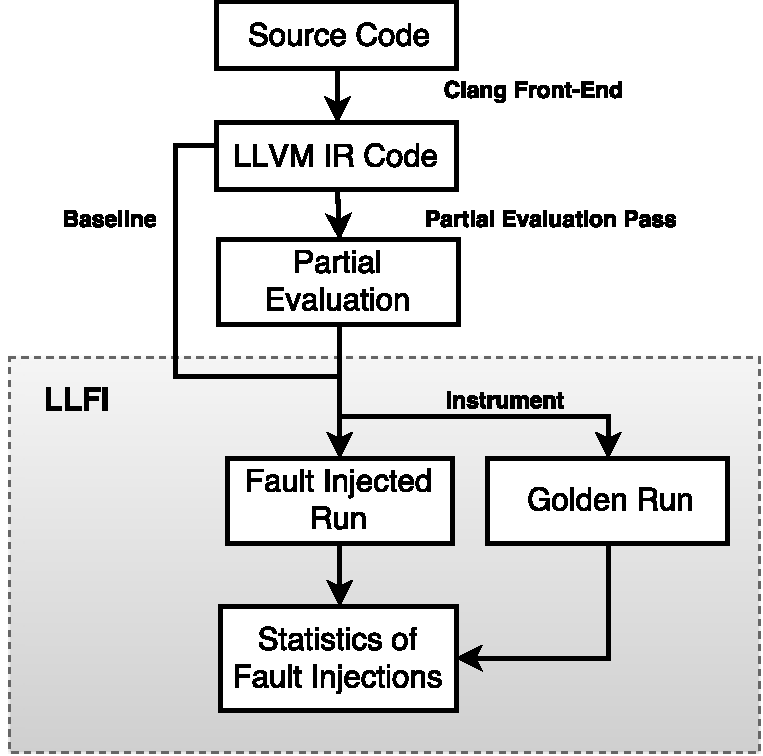
\includegraphics[keepaspectratio=true,width=0.8\columnwidth]{Evaluation_System}
  \caption{System Block Diagram of Evaluation Experimental Setup}
  \label{fig:evaluation_sys}
\end{figure}

In the algorithms we selected, we anticipate that they will tolerate singular faults.
For example, we expect DepthCount to tolerate pointer errors at individual tree nodes, without impacting traversal of the remaining tree.
However, the specialized forms of the program may eliminate such features upon compile time optimization.
Thus, we aim to measure and compare the error resiliencies of the baseline and its partial evaluation respectively.

We utilize the LLVM based fault injector, LLFI~\cite{LLFI} to carry out the experimentation.
LLFI injects software implemented faults into the program IR by modifying instruction or register values of the program at runtime.
It offers a range of simulated hardware and software faults that model real-world conditions~\cite{V2005}.
In this study, we select the following faults: bit flips, stuck-at-0, return value corruption, function call corruption, and invalid pointer.
Bit flips represent transient hardware faults, while stuck-at-0 represents permanent hardware faults. 
The rest of the faults represent transient software faults that occur as a result of a data corruption.
We omit permanent software faults in this study as discussed in Section~\ref{sec:fault_model}.

The injected faults are uniformly distributed throughout the program code.
Table~\ref{tab:faulttypes} describes how LLFI injects each fault.
We consider only activated faults, or those in which the modified data is read by the program, when measuring the fault outcome rate.


\begin{table}[htbp]
\small{
\begin{center}
    \begin{tabular}{|p{0.1cm}|p{2.4cm}|p{5cm}|}
    \hline
     & \textbf{Fault Type} & \textbf{LLFI Implementation} \\ \hline
    A & Bit Flip & Randomly flips a single bit in an arbitrary data value computed in the program  \\ \hline
    B & Stuck at 0 & Randomly sets a single bit to 0 in an arbitrary data value computed in the program  \\ \hline
    C & Return Value Corruption & Randomly corrupts the return value of a function call \\ \hline
    D & Function Call Corruption & Randomly corrupts the source register (i.e., parameter) of a function call \\ \hline
    E & Invalid Pointer & Randomly corrupts the returned pointer from malloc and calloc\\ \hline
    \hline
    \end{tabular}
    \end{center}
    }
    \caption{Description of faults injected using LLFI}
    \label{tab:faulttypes}
\end{table}
 

After running the experiment, we group and classify the results of the faulty program trials according to their failure outcome modes.
We determine whether the observations hold across failure modes and fault types. 
We make the following hypothesis with respect to the failure outcome rates.

\begin{hyp}
  \label{hyp:hypothesis}
The mean fault outcome rate $(f_p)$ of a program's partial evaluation is statistically equal to the mean fault outcome rate of the original program $(f_0$).
\end{hyp}

To realize this, we perform a two-sample t-test to determine whether the means are statistically equivalent to each other, within a 95\% confidence interval ($\delta_0$).
Our hypothesis expressed in formal terms is $H_1: f_0 - f_p < \delta_0 $.

In addition to measuring error resilience, we also measure the number of IR instructions and the execution times of the partial evaluation and the original program respectively.
This allows us to compute the speedup factor, $\psi$, defined as
\begin{align*}
\psi = \frac{P_t}{P'_t}
\end{align*}

where $P_t$ and $P'_t$ are the execution durations of the original program, and its partial evaluation respectively.
The speedup factor provides an approximate measure of the extent of code optimization and allows us to reason about correlations between partial evaluations and error resilience.


\subsection{Results}
\label{sec:results}

We make the following observations from our set of fault injection experiments.

\begin{obs}
  \label{obs:faultoutcomes}
  On average, the fault outcome rates of a program and its partial evaluation are not statistically different from each other.
\end{obs}

Figures [\ref{fig:BinaryTree_8}-\ref{fig:Mandelbrot_1000}] show the fault outcome rates of the original program $(f_0)$ and its partial evaluation $(f_p)$ respectively for each fault type.
These results are shown for three different inputs (values of N) over each of the three benchmarks, across 1000 fault injections.  
In the graphs, $f_0$ is denoted as P and $f_p$ is denoted as PE.
The fault outcome rates are further divided into their failure modes: SDCs and Crash/Hangs.
The error bounds denote the standard error margins of the reported fault outcome rates.

Overall, we find that $f_0$ and $f_p$ are within the standard error margin in most of the fault injection runs.
However, many exceptions to this trend are present.
The most significant differences can be observed in the SDC and Crash/Hang rates of Return Value Corruptions in Figure~\ref{fig:Fannkuch_8} and the SDC rates among all fault types in Figure~\ref{fig:Mandelbrot_10} and Figure~\ref{fig:Mandelbrot_100}.

Tables [\ref{tab:DepthCount_TTest}-\ref{tab:Mandelbrot_TTest}] show the results of the two sample t-test conducted on the mean SDC and Crash/Hang failure outcomes for each fault type.
We did not perform a t-test on Crash/Hang failure outcomes for Mandelbrot as the means were too small.
Here, $n_0$ and $n_p$ represent the absolute mean number of faulty runs that result in failures during the 1000 fault injections. 

Since our confidence interval is 95\%, $\alpha=0.05$.
If the p value is less than the alpha value, our hypothesis is rejected.
In a majority of the entries, our hypothesis statistically holds.
It also appears that the fault resiliencies do not statistically differ when programs are subject to a greater input load.
In the case of Mandelbrot, the gap between fault resiliencies of the program and its partial evaluation reduced in N=1000 compared to N=10.

\begin{figure}[htbp]
  \centering
  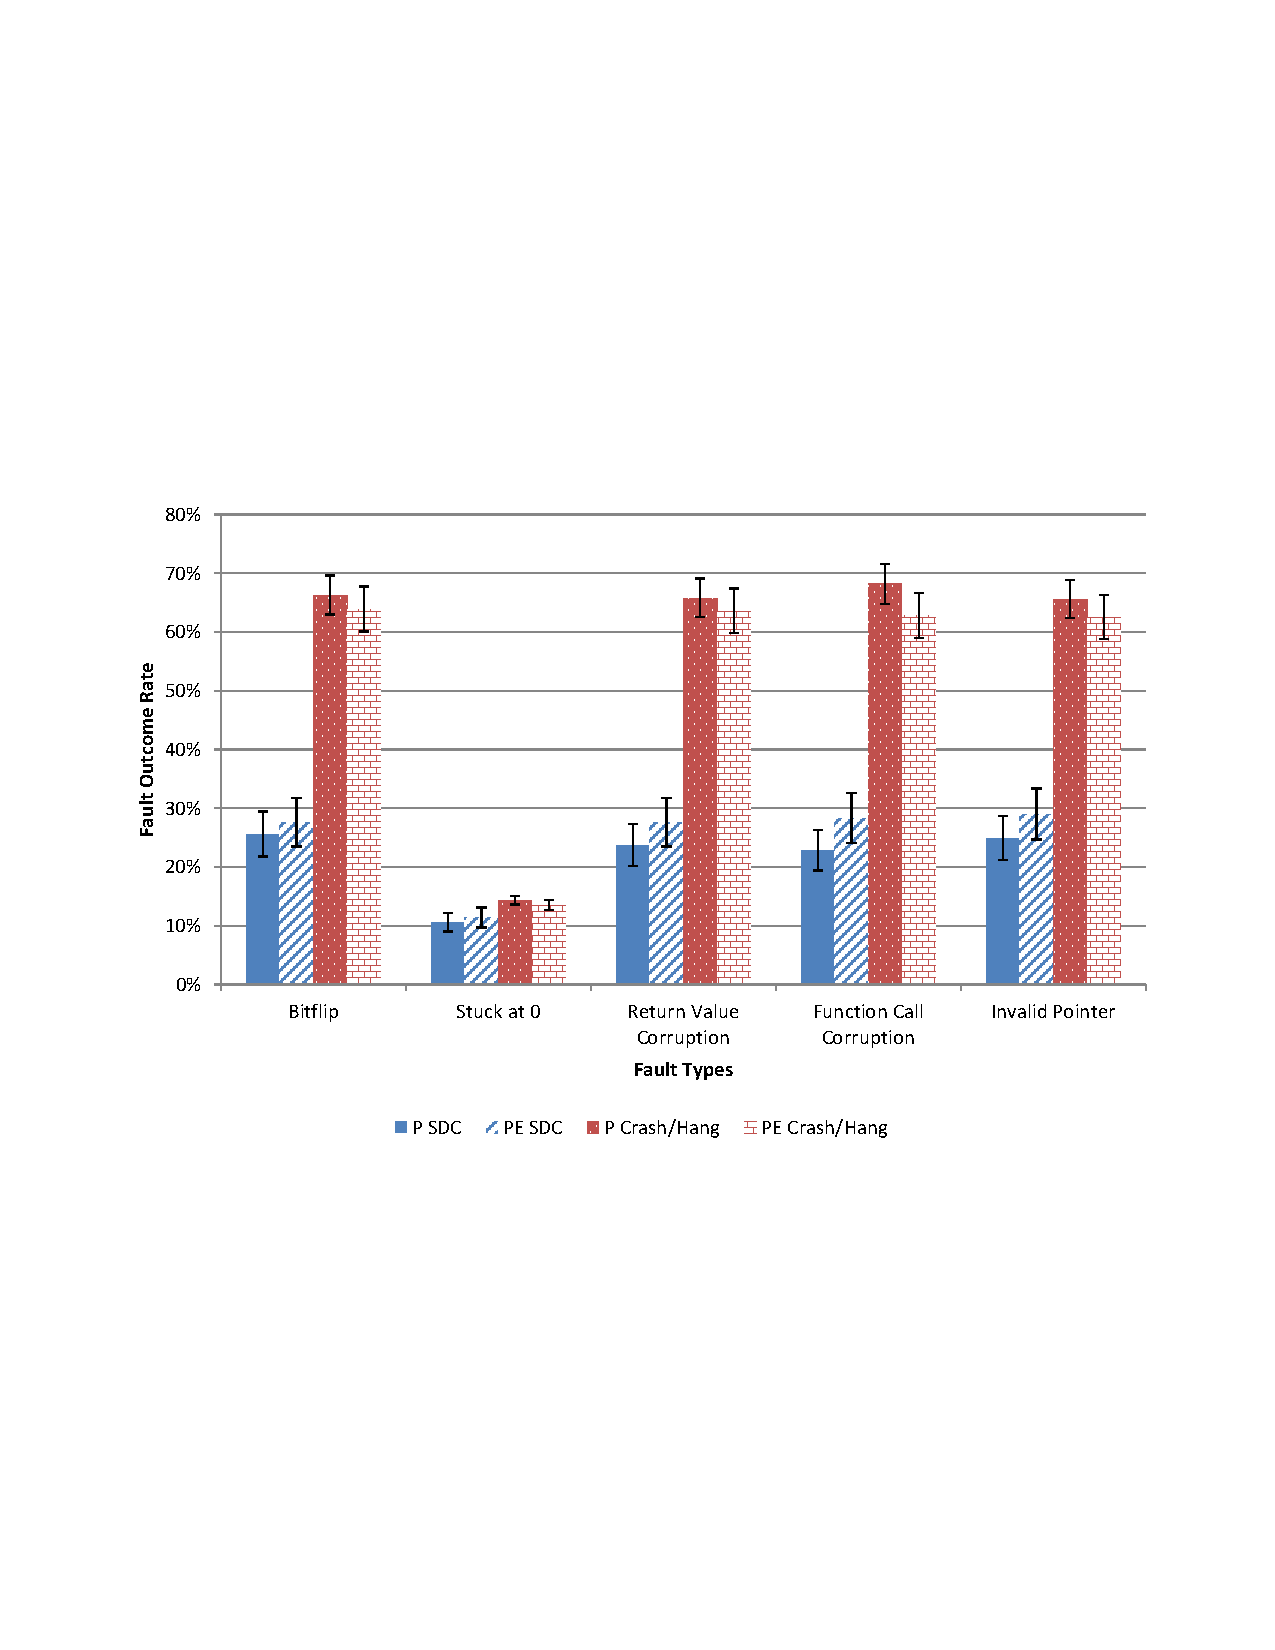
\includegraphics[keepaspectratio=true,width=\columnwidth]{BinaryTree_8}
  \caption{Fault Outcome Rates of DepthCount, with N=8}
  \label{fig:BinaryTree_8}
\end{figure}

\begin{figure}[htbp]
  \centering
  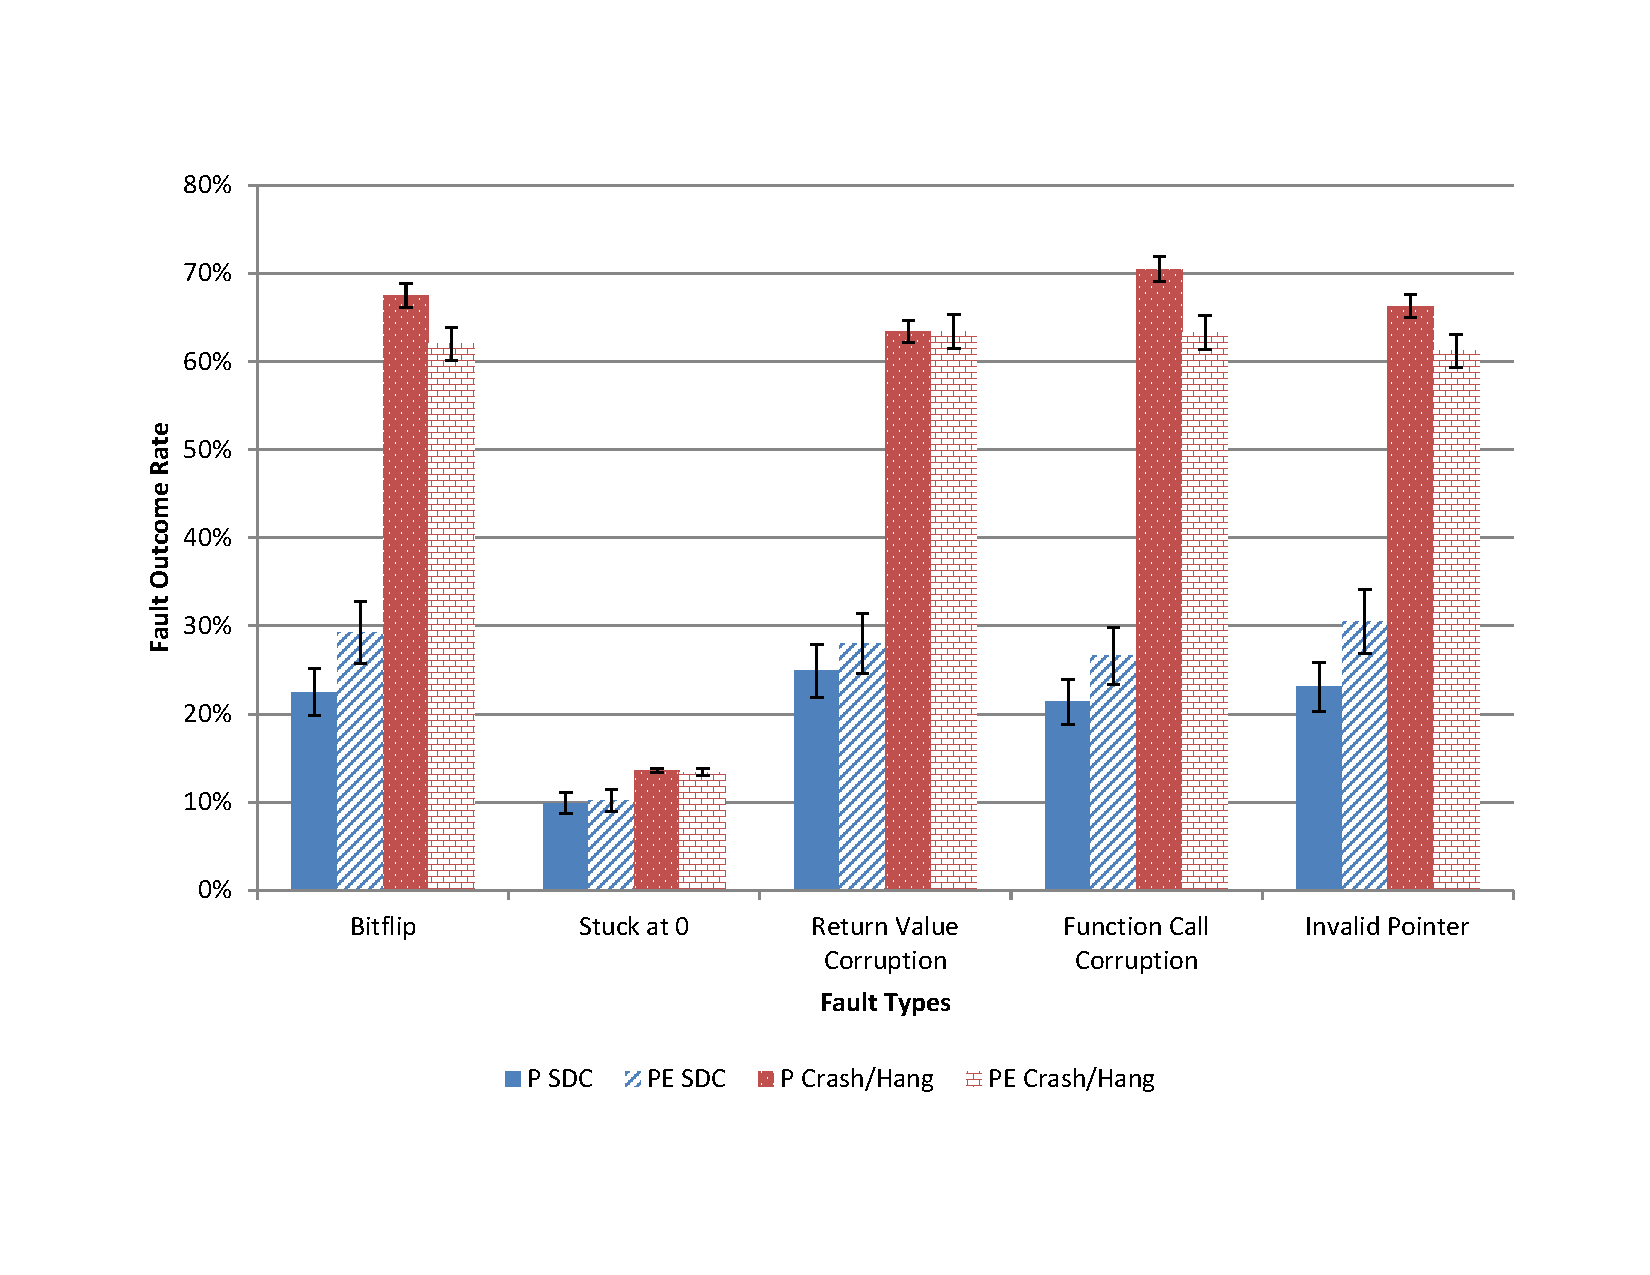
\includegraphics[keepaspectratio=true,width=\columnwidth]{BinaryTree_10}
  \caption{Fault Outcome Rates of DepthCount, with N=10}
  \label{fig:BinaryTree_10}
\end{figure}

\begin{figure}[htbp]
  \centering
  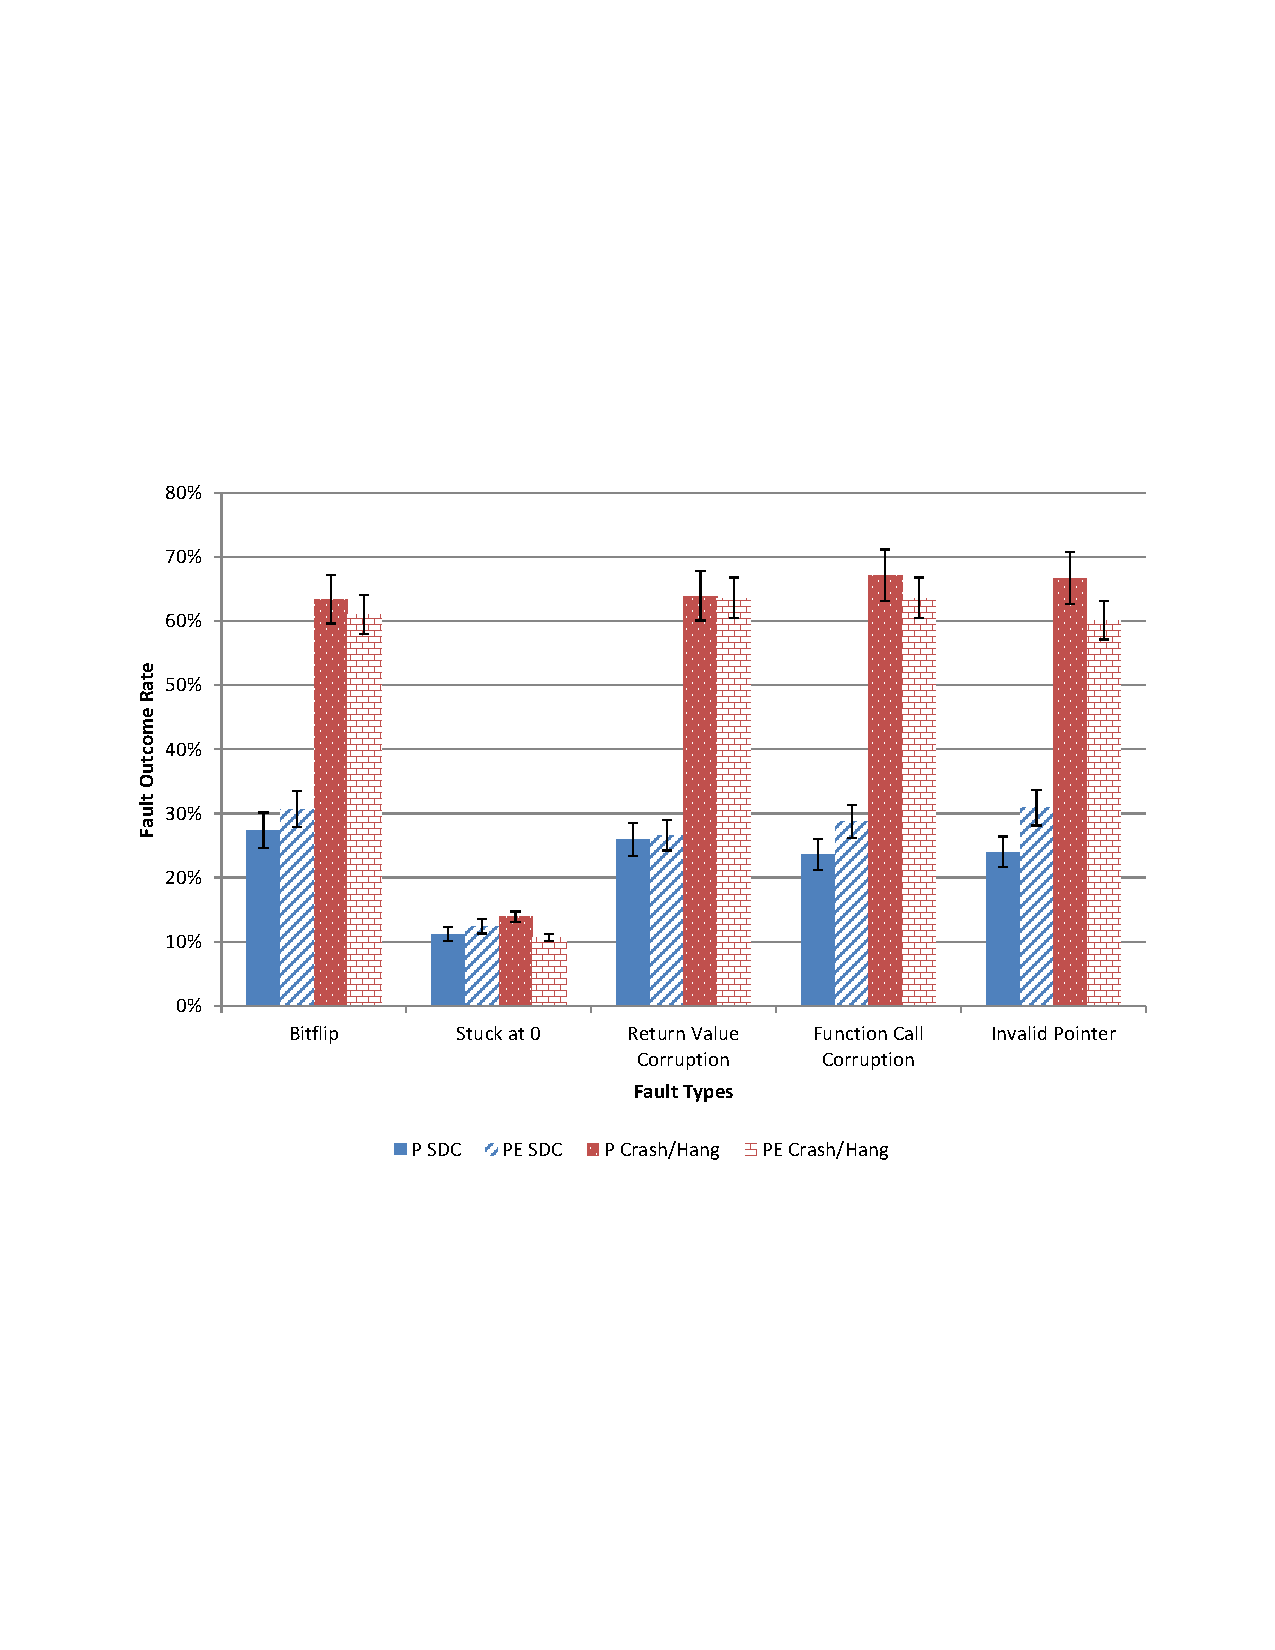
\includegraphics[keepaspectratio=true,width=\columnwidth]{BinaryTree_12}
  \caption{Fault Outcome Rates of DepthCount, with N=12}
  \label{fig:BinaryTree_12}
\end{figure}

\begin{figure}[htbp]
  \centering
  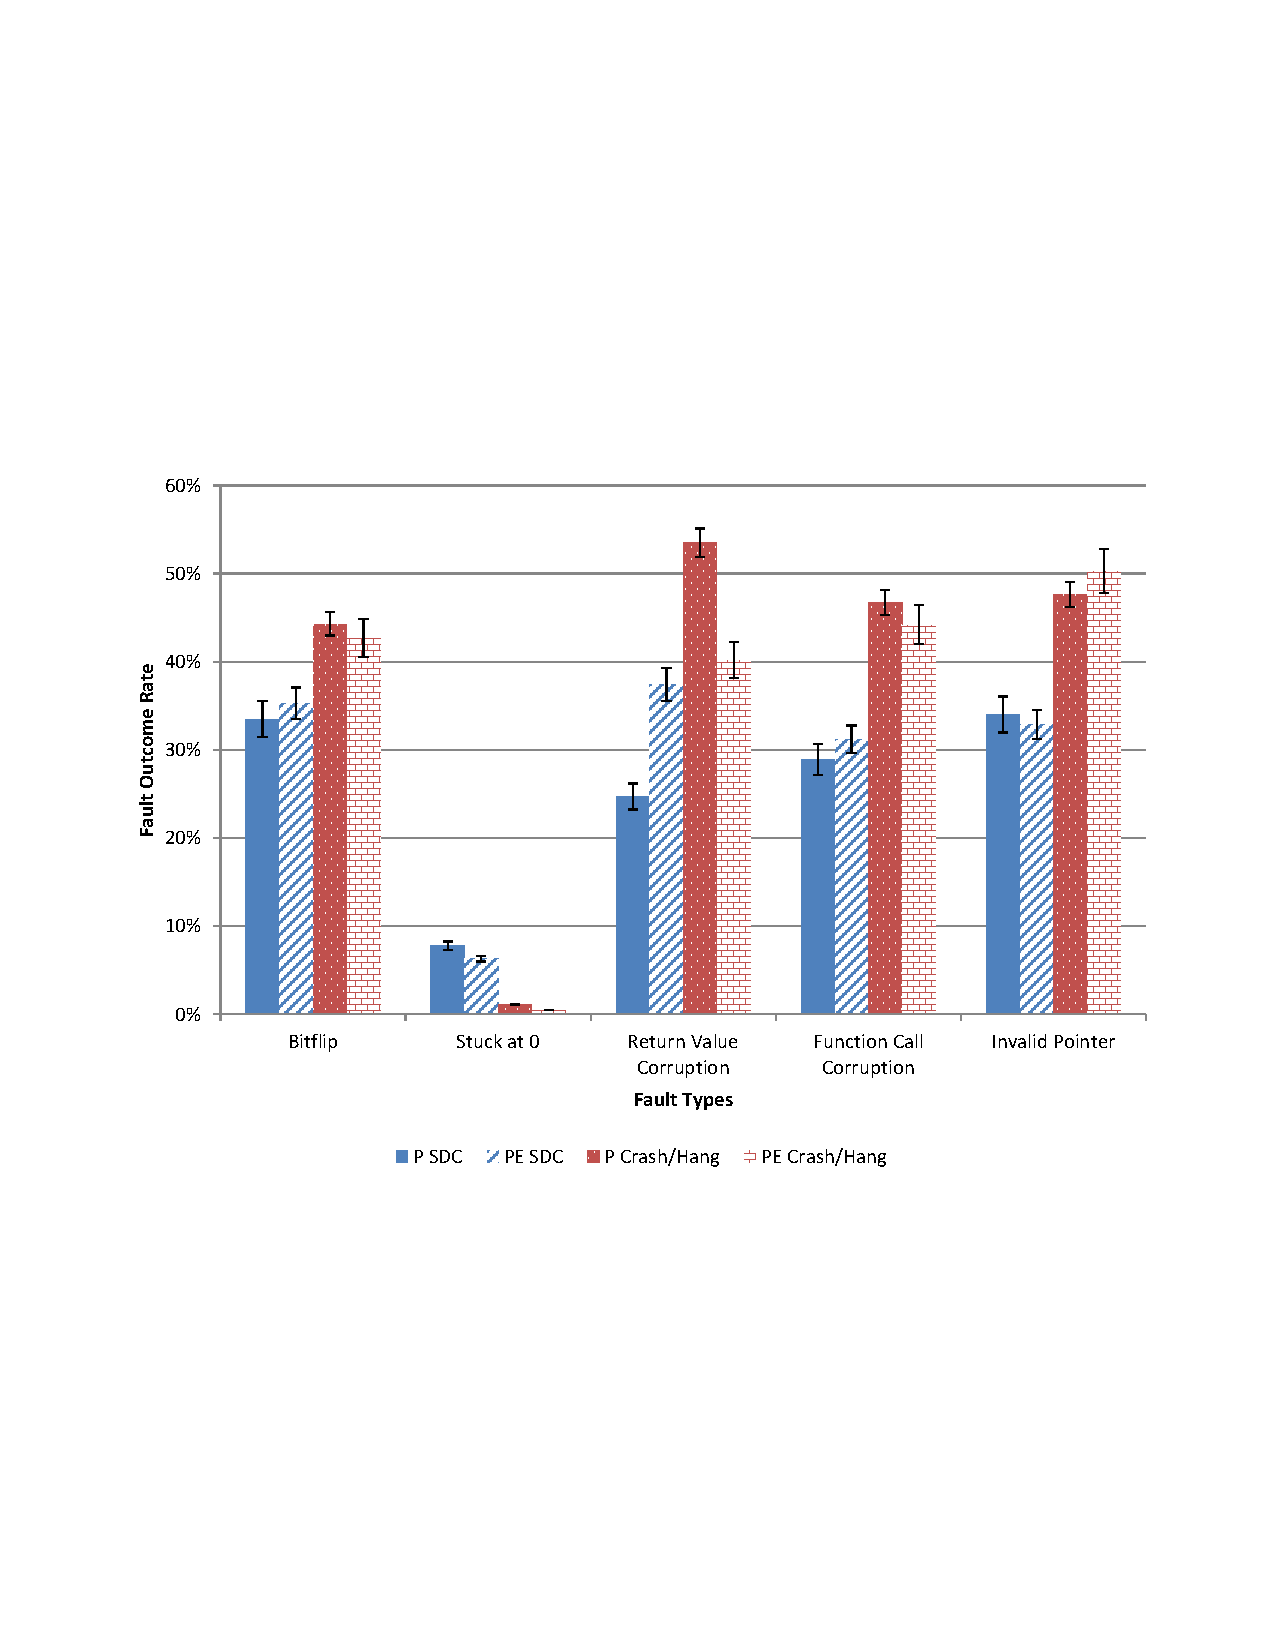
\includegraphics[keepaspectratio=true,width=\columnwidth]{Fannkuch_8}
  \caption{Fault Outcome Rates of Fannkuch, with N=8}
  \label{fig:Fannkuch_8}
\end{figure}

\begin{figure}[htbp]
  \centering
  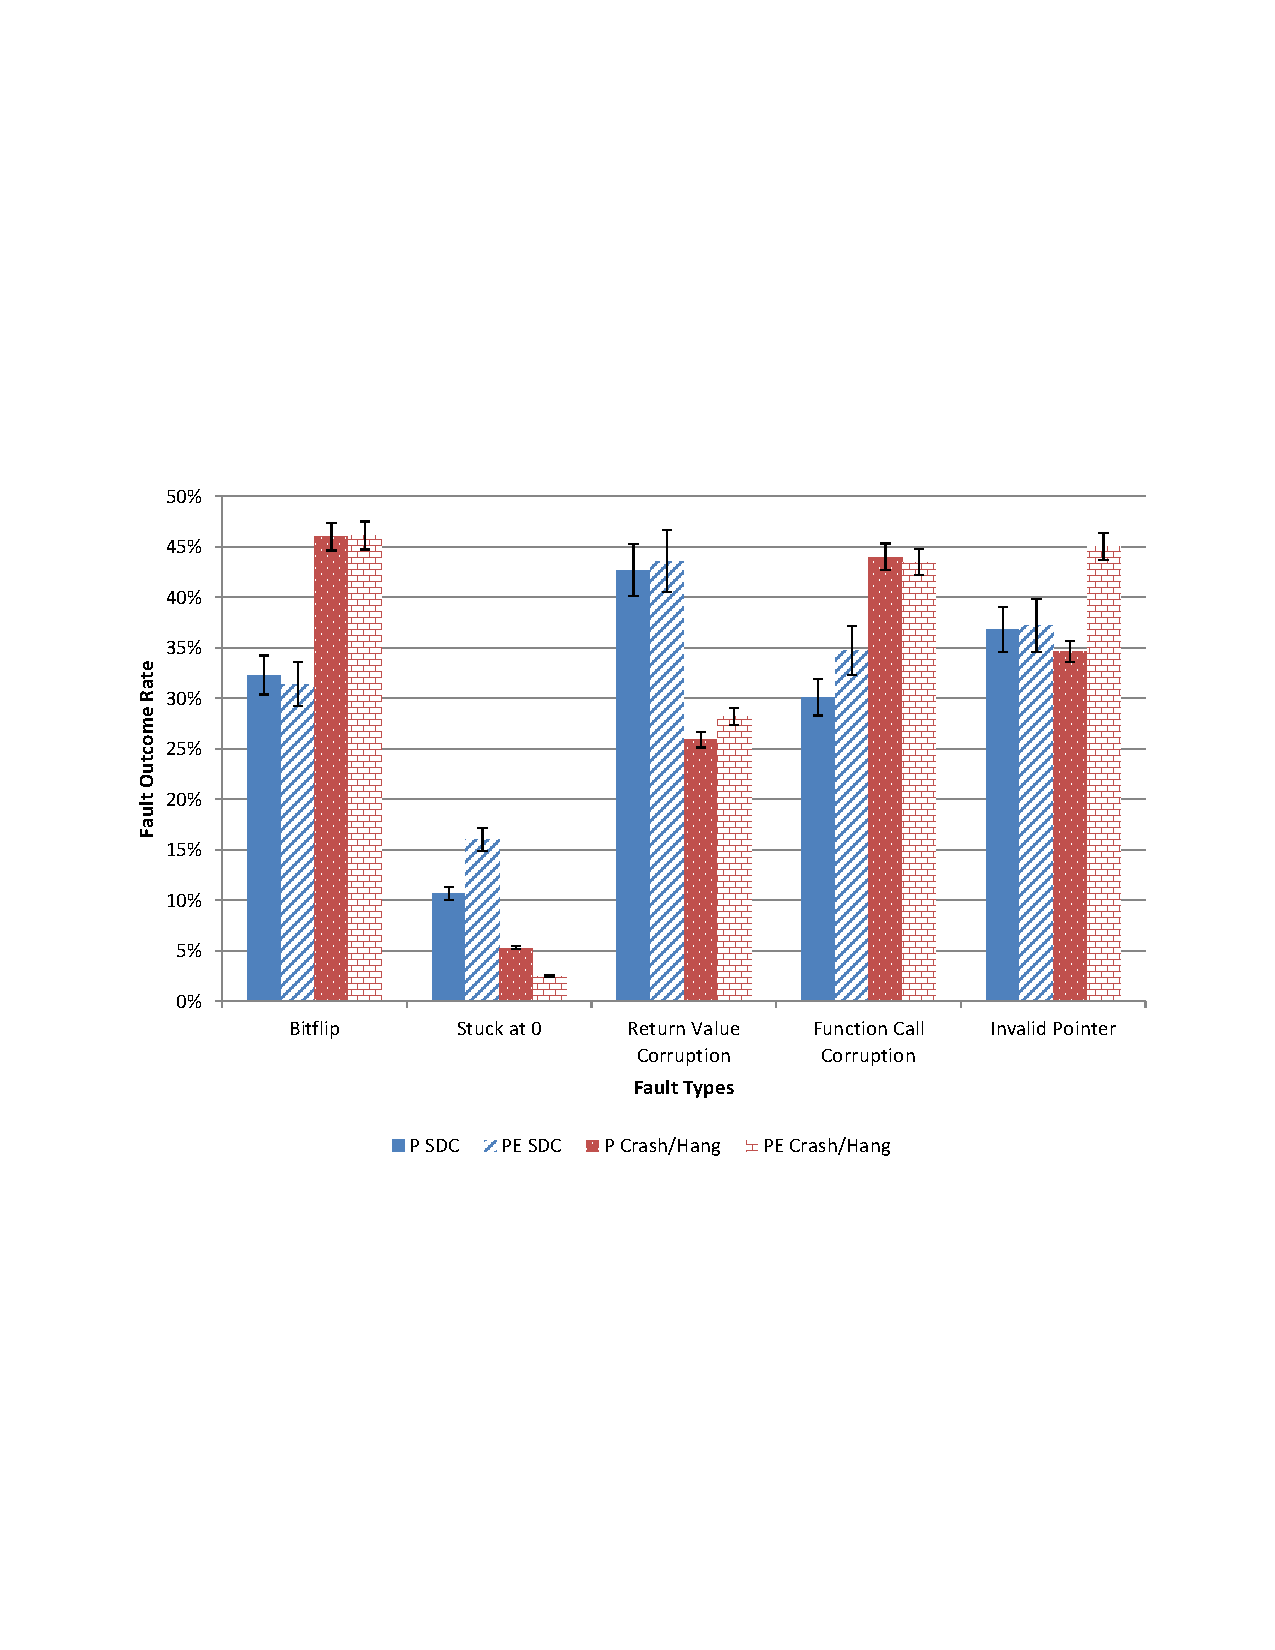
\includegraphics[keepaspectratio=true,width=\columnwidth]{Fannkuch_9}
  \caption{Fault Outcome Rates of Fannkuch, with N=9}
  \label{fig:Fannkuch_9}
\end{figure}

\begin{figure}[htbp]
  \centering
  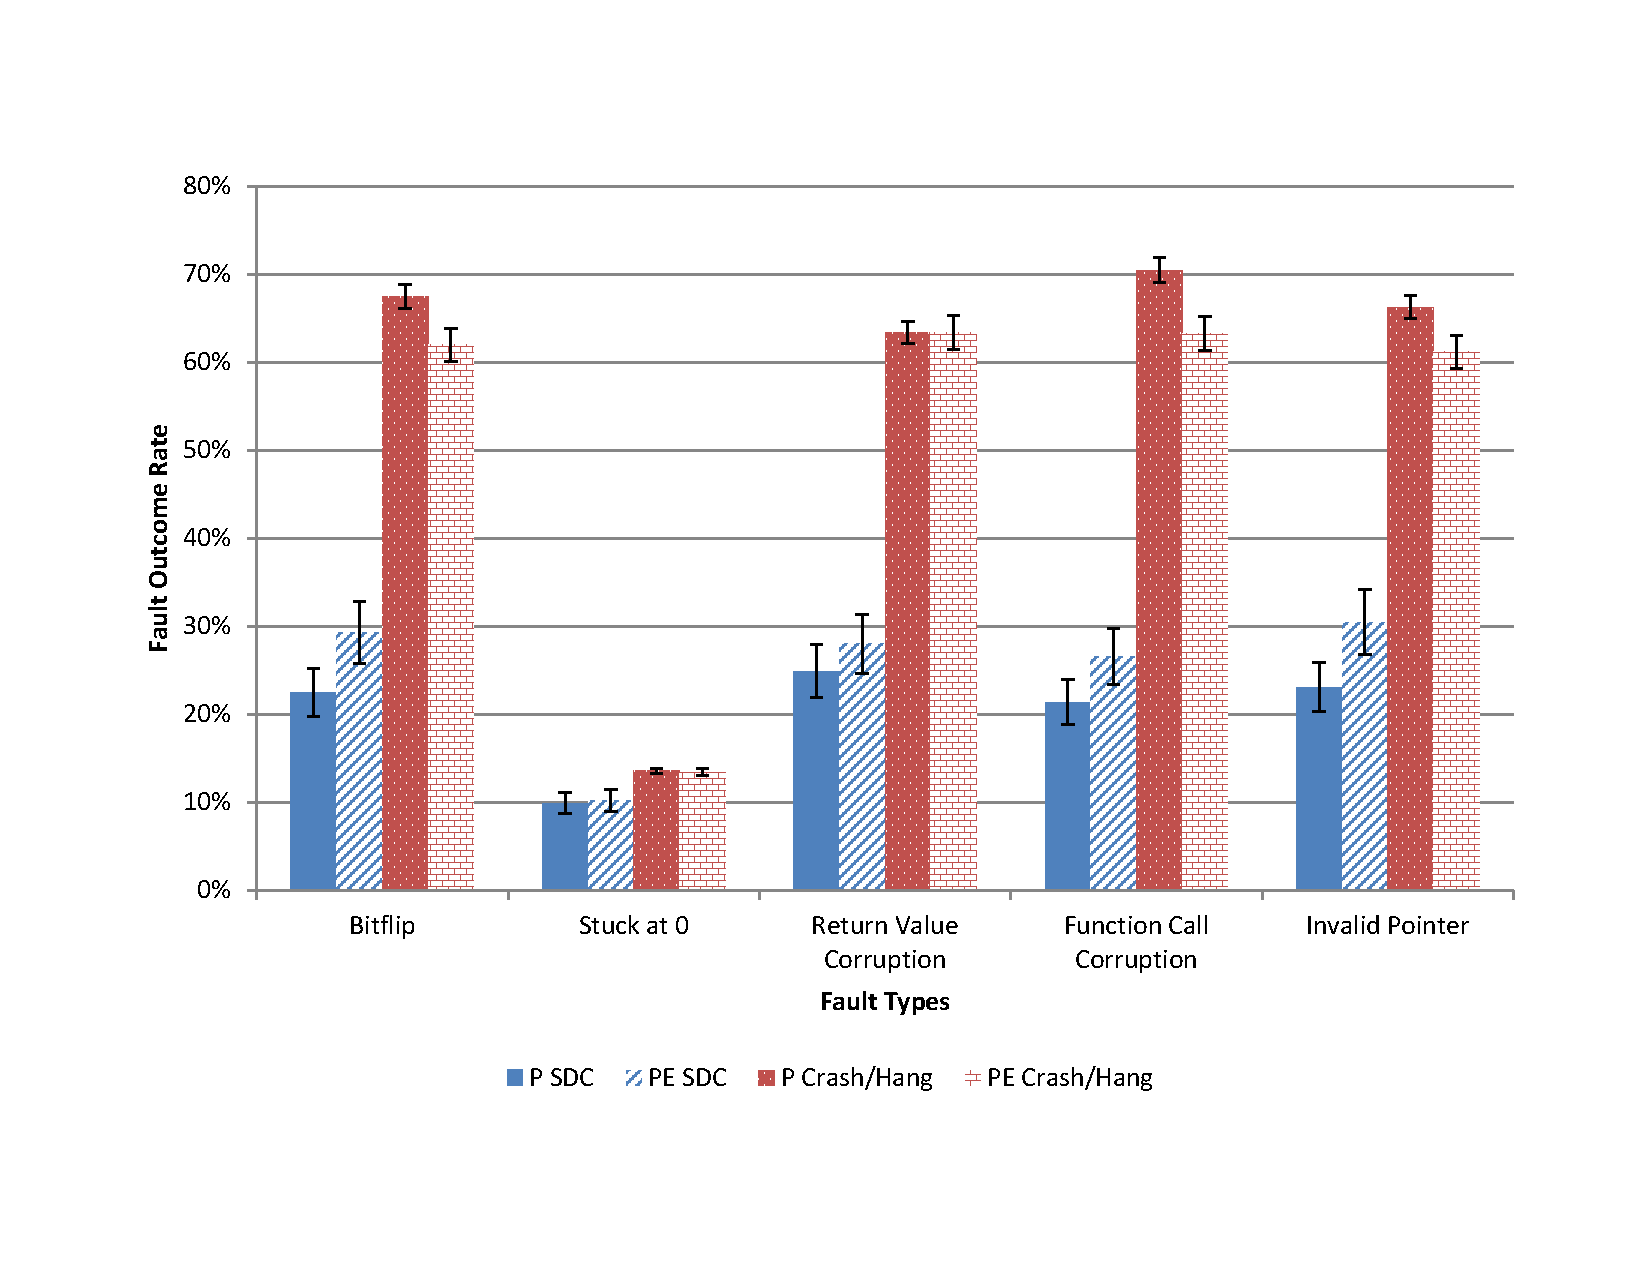
\includegraphics[keepaspectratio=true,width=\columnwidth]{Fannkuch_10}
  \caption{Fault Outcome Rates of Fannkuch, with N=10}
  \label{fig:Fannkuch_10}
\end{figure}

\begin{figure}[htbp]
  \centering
  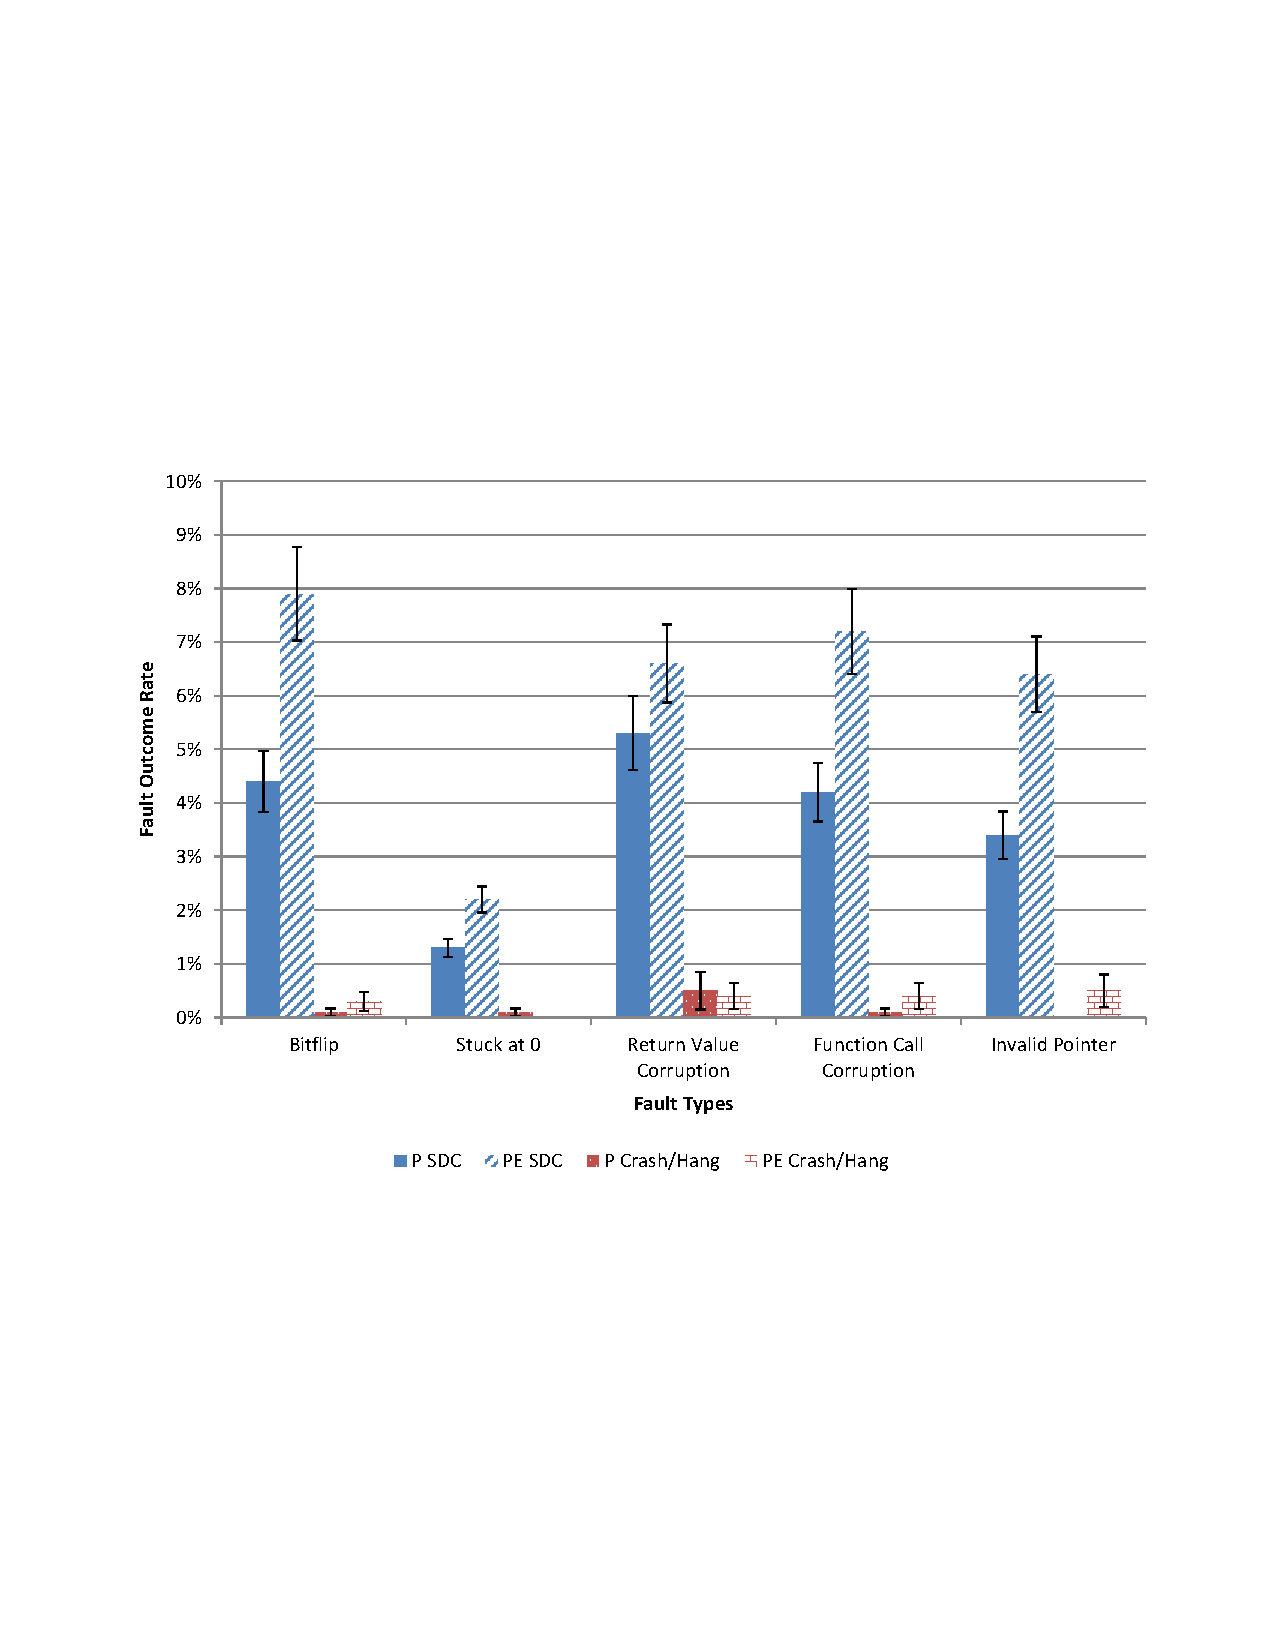
\includegraphics[keepaspectratio=true,width=\columnwidth]{Mandelbrot_10}
  \caption{Fault Outcome Rates of Mandelbrot, with N=10}
  \label{fig:Mandelbrot_10}
\end{figure}

\begin{figure}[htbp]
  \centering
  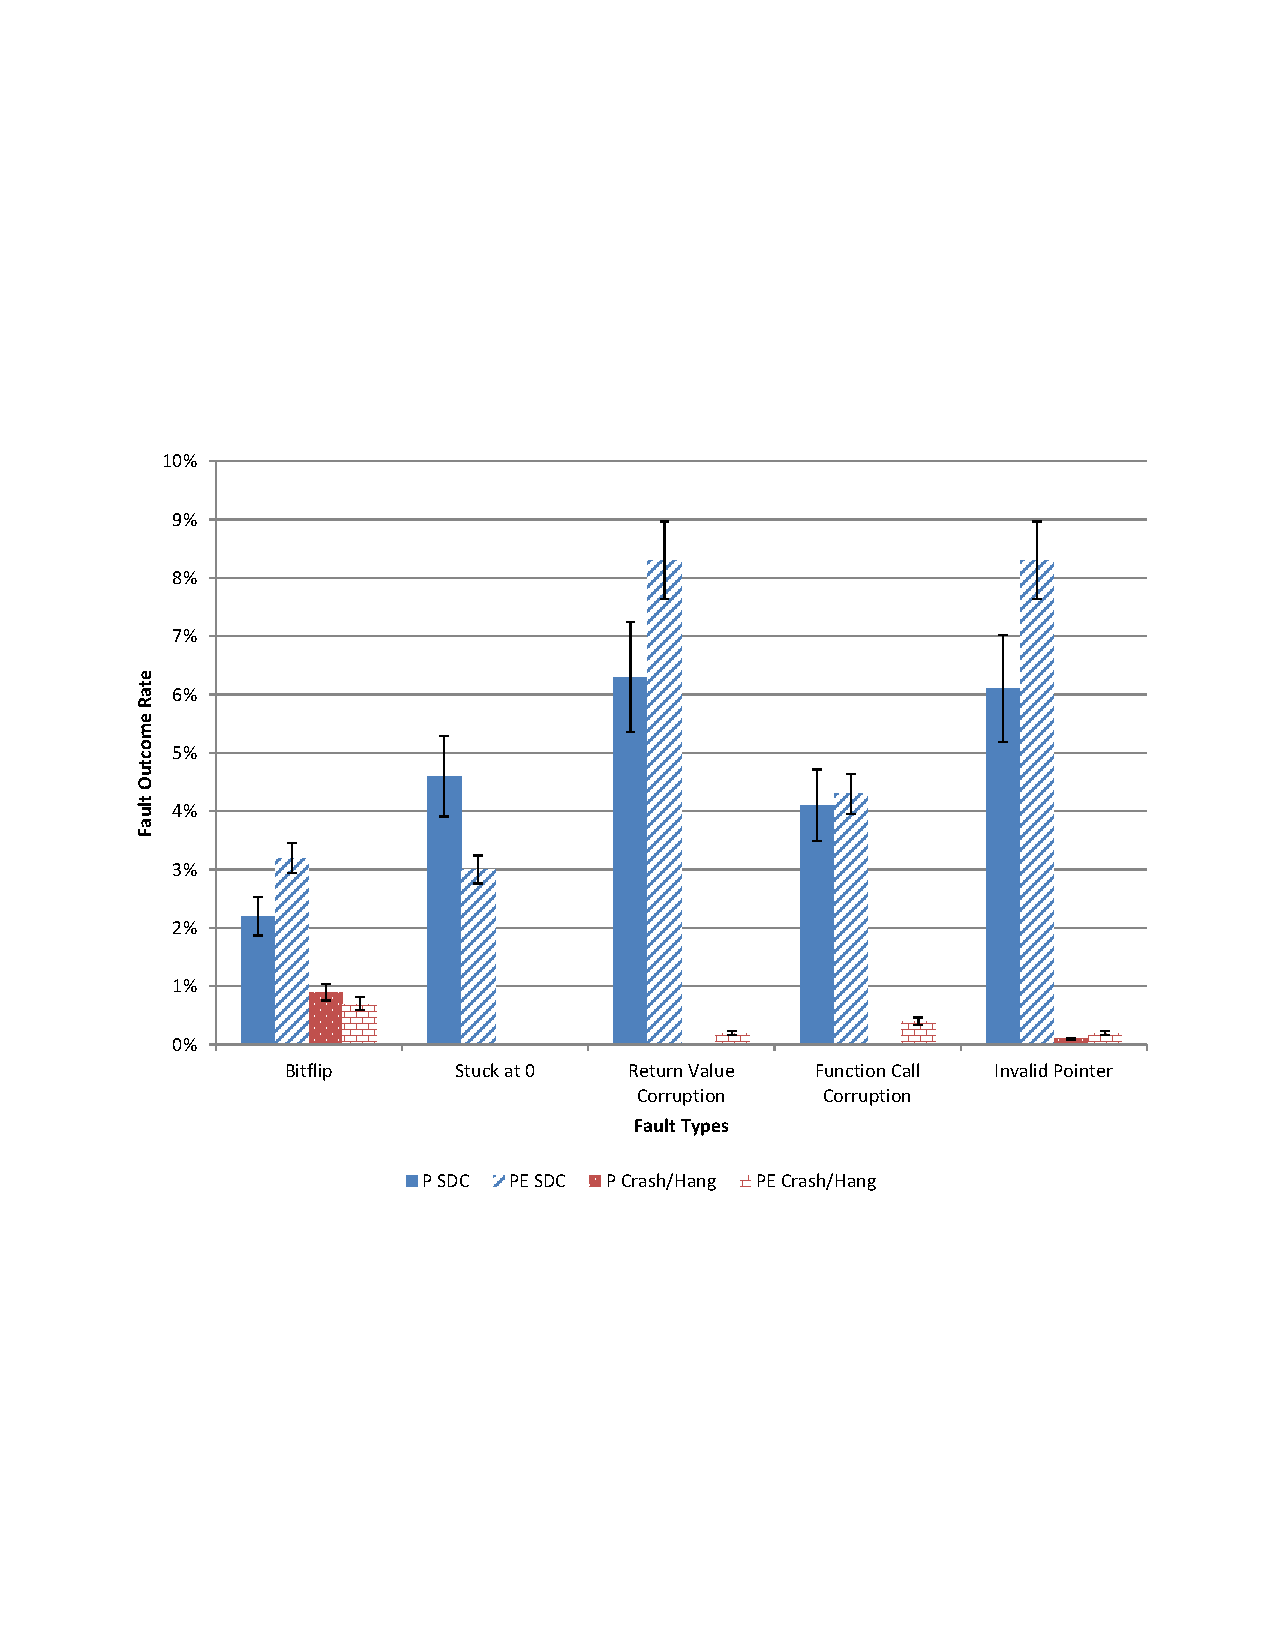
\includegraphics[keepaspectratio=true,width=\columnwidth]{Mandelbrot_100}
  \caption{Fault Outcome Rates of Mandelbrot, with N=100}
  \label{fig:Mandelbrot_100}
\end{figure}

\begin{figure}[htbp]
  \centering
  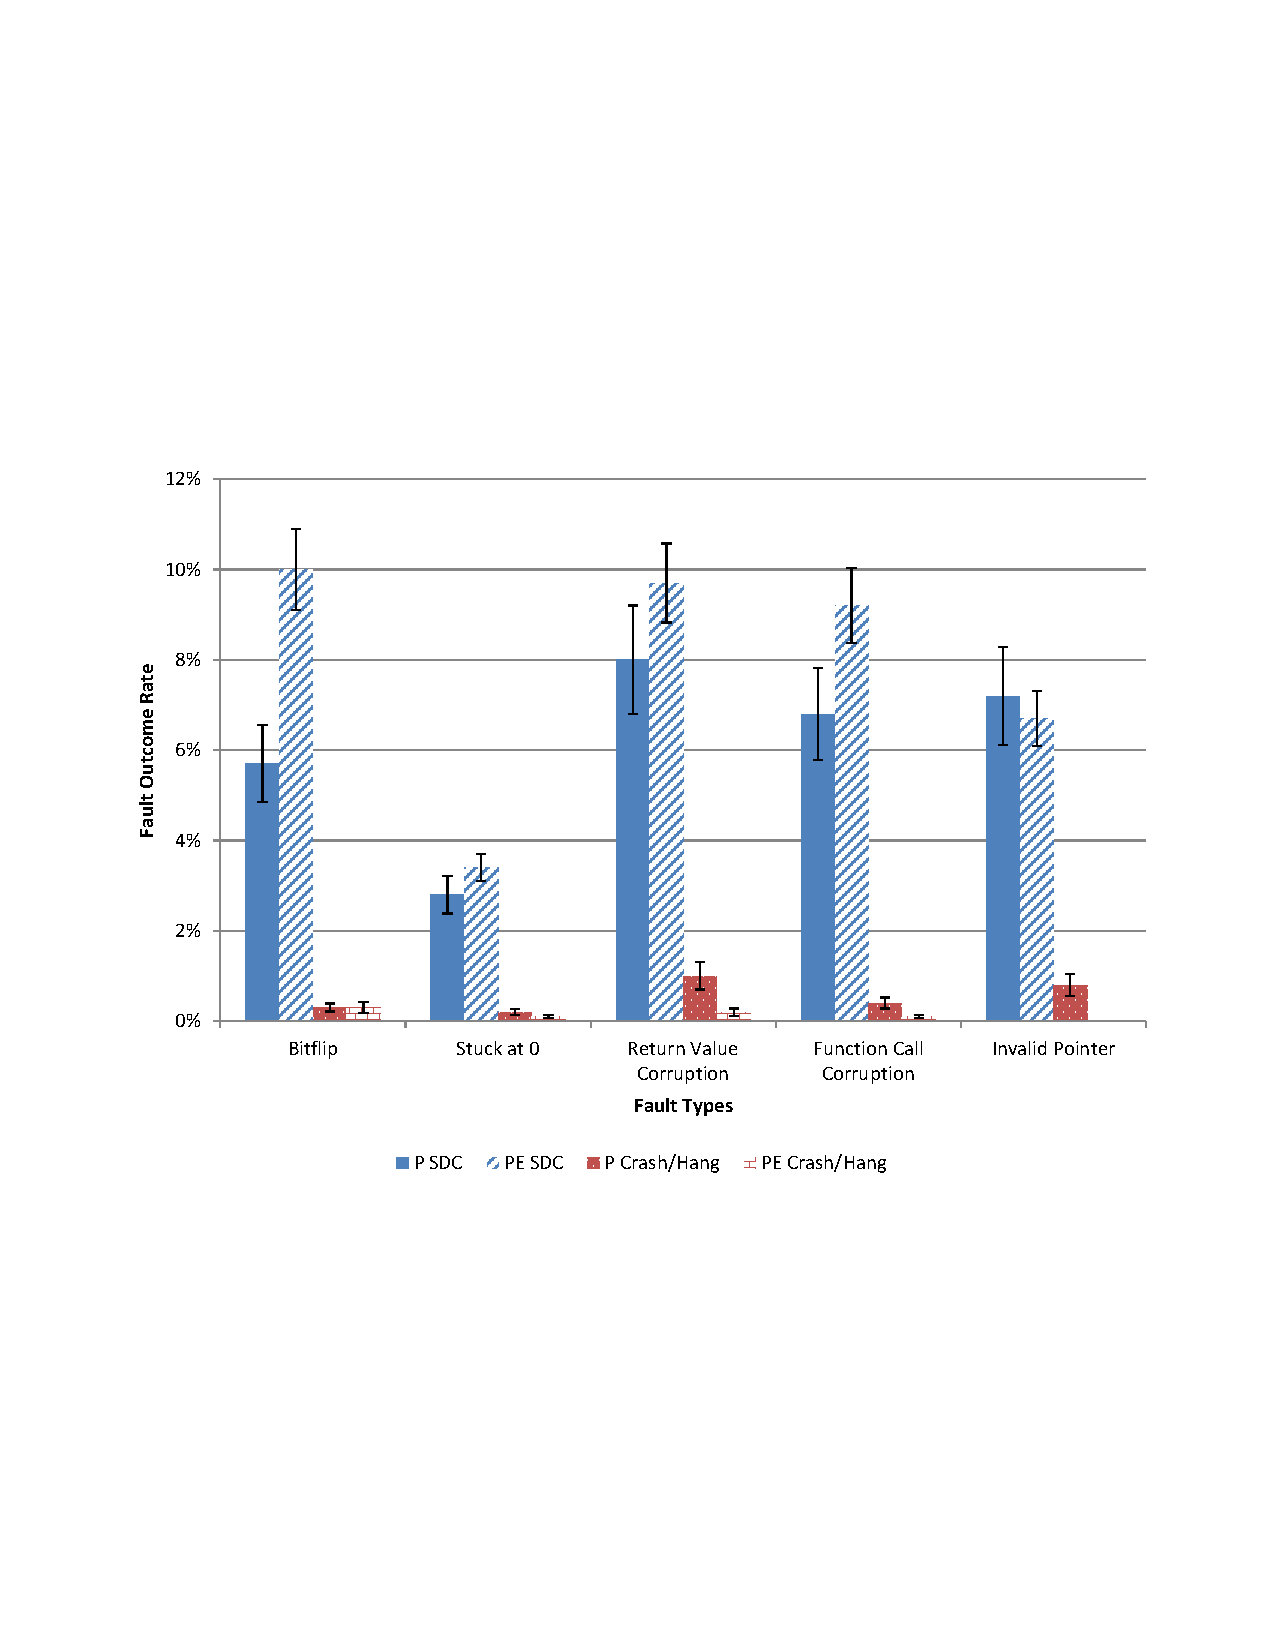
\includegraphics[keepaspectratio=true,width=\columnwidth]{Mandelbrot_1000}
  \caption{Fault Outcome Rates of Mandelbrot, with N=1000}
  \label{fig:Mandelbrot_1000}
\end{figure}


\begin{table}[htbp]
\small{
\begin{center}
    \begin{tabular}{|p{0.7cm}|c|c|c|c|c|}
    \hline
    \textbf{Input} & \textbf{Fault} & \textbf{$n_0$ (SE)} & \textbf{$n_p$ (SE)} & \textbf{t} & \textbf{p} \\ \hline
    \multirow{5}{*}{8}
    & A & 256(13.80) & 276(14.14) & 1.0122 & 0.3115 \\
	& B & 106(9.73) & 114(10.05) & 0.5719 & 0.5675 \\
 	& C & 237(13.45) & 276(14.14) & 1.9984 & 0.0458 \\
 	& D & 228(13.27) & 283(14.24) & 2.8256 & 0.0048 \\
 	& E & 249(13.67) & 290(14.35) & 2.0687 & 0.0387 \\ \hline
    \multirow{5}{*}{10}
    & A & 225(13.21) & 293(14.39) & 3.4811 & $<$0.001 \\
	& B & 99(9.44) & 102(9.57) & 0.2232 & 0.8234 \\
 	& C & 249(13.67) & 280(14.20) & 1.5728 & 0.1159 \\
 	& D & 214(12.97) & 266(13.97) & 2.7279 & 0.0064 \\
 	& E & 231(13.33) & 305(14.56) & 3.7487 & $<$0.001 \\ \hline
 	\multirow{5}{*}{12}
    & A & 274(14.10) & 307(14.59) & 1.6264 & 0.1040 \\
	& B & 112(9.97) & 124(10.42) & 0.8321 & 0.4055 \\
 	& C & 259(13.85) & 266(13.97) & 0.3558 & 0.7220 \\
 	& D & 236(13.43) & 287(14.30) & 2.5997 & 0.0094 \\
 	& E & 240(13.51) & 309(14.61) & 3.4675 & $<$0.001 \\ \hline
    \hline
    \end{tabular}
    \end{center}
    }
    \caption{T-Test Results for DepthCount SDC Fault Outcomes}
    \label{tab:DepthCount_TTest}
\end{table}

\begin{table}[htbp]
\small{
\begin{center}
    \begin{tabular}{|p{0.7cm}|c|c|c|c|c|}
    \hline
    \textbf{Input} & \textbf{Fault} & \textbf{$n_0$ (SE)} & \textbf{$n_p$ (SE)} & \textbf{t} & \textbf{p} \\ \hline
    \multirow{5}{*}{8}
    & A & 663(14.95) & 639(15.19) & 1.1261 & 0.2603 \\
	& B & 143(11.07) & 135(10.81) & 0.5170 & 0.6052 \\
 	& C & 658(15.00) & 636(15.22) & 1.0295 & 0.3034 \\
 	& D & 682(14.73) & 628(15.28) & 2.5443 & 0.0110 \\
 	& E & 656(15.02) & 625(15.31) & 1.4454 & 0.1485 \\ \hline
    \multirow{5}{*}{10}
    & A & 675(14.81) & 620(15.35) & 2.5786 & 0.0100 \\
	& B & 136(10.84) & 134(10.77) & 0.1309 & 0.8959 \\
 	& C & 634(15.23) & 634(15.23) & 0.0000 & 1.0000 \\
 	& D & 705(14.42) & 633(15.24) & 3.4317 & $<$0.001 \\
 	& E & 663(14.95) & 612(15.41) & 2.3754 & 0.0176 \\ \hline
 	\multirow{5}{*}{12}
    & A & 634(15.23) & 610(15.42) & 1.1074 & 0.2683 \\
	& B & 139(10.94) & 107(9.78) & 2.1807 & 0.0293 \\
 	& C & 639(15.19) & 636(15.22) & 0.1395 & 0.8891 \\
 	& D & 671(14.86) & 636(15.22) & 1.6454 & 0.1000 \\
 	& E & 667(14.90) & 601(15.49) & 3.0708 & 0.0022 \\ \hline
    \hline
    \end{tabular}
    \end{center}
    }
    \caption{T-Test Results for DepthCount Crash Fault Outcomes}
    \label{tab:DepthCount_Crash_TTest}
\end{table}

\begin{table}[htbp]
\small{
\begin{center}
    \begin{tabular}{|p{0.7cm}|c|c|c|c|c|}
    \hline
    \textbf{Input} & \textbf{Fault} & \textbf{$n_0$ (SE)} & \textbf{$n_p$ (SE)} & \textbf{t} & \textbf{p} \\ \hline
    \multirow{5}{*}{8}
    & A & 335(14.93) & 353(15.11) & 0.8474 & 0.3969 \\
	& B & 78(8.48) & 63(7.68) & 1.3111 &  0.1900 \\
 	& C & 247(13.64) & 374(15.30) & 6.1959 & $<$0.001 \\
 	& D & 289(14.33) & 312(14.65) & 1.1223 & 0.2619 \\
 	& E & 340(14.98) & 329(14.86) & 0.5213 & 0.6022 \\ \hline
    \multirow{5}{*}{9}
    & A & 323(14.79) & 314(14.68) & 0.4319 & 0.6659 \\
	& B & 107(9.78) & 160(11.59) & 3.4949 & $<$0.001 \\
 	& C & 427(15.64) & 436(15.68) & 0.4064 & 0.6845 \\
 	& D & 301(14.51) & 347(15.05) & 2.2004 & 0.0279 \\
 	& E & 368(15.25) & 372(15.28) & 0.1853 & 0.8530 \\ \hline
 	\multirow{5}{*}{10}
    & A & 251(13.71) & 314(14.68) & 3.1364 & 0.0017 \\
	& B & 7(3.64) & 74(8.28) & 7.4076 & $<$0.001 \\
 	& C & 416(15.59) & 300(14.49) & 5.4501 & $<$0.001 \\
 	& D & 180(12.15) & 293(14.39) & 6.0000 & $<$0.001 \\
 	& E & 232(13.35) & 187(12.33) & 2.4762 & 0.0134 \\ \hline
    \hline
    \end{tabular}
    \end{center}
    }
    \caption{T-Test Results for Fannkuch SDC Fault Outcomes}
    \label{tab:Fannkuch_TTest}
\end{table}

\begin{table}[htbp]
\small{
\begin{center}
    \begin{tabular}{|p{0.7cm}|c|c|c|c|c|}
    \hline
    \textbf{Input} & \textbf{Fault} & \textbf{$n_0$ (SE)} & \textbf{$n_p$ (SE)} & \textbf{t} & \textbf{p} \\ \hline
    \multirow{5}{*}{8}
    & A & 443(15.71) & 427(15.64) & 0.7218 & 0.4705 \\
	& B & 11(3.30) & 5(2.23) & 1.5065 & 0.1321 \\
 	& C & 535(15.77) & 402(15.50) & 6.0148 & $<$0.001 \\
 	& D & 467(15.78) & 442(15.70) & 1.1231 & 0.2615 \\
 	& E & 476(15.79) & 503(15.81) & 1.2083 & 0.2271 \\ \hline
    \multirow{5}{*}{9}
    & A & 460(15.76) & 461(15.76) & 0.0449 & 0.9642 \\
	& B & 53(7.08) & 25(4.94) & 3.2433 & 0.0012 \\
 	& C & 259(13.85) & 282(14.23) & 1.1583 & 0.2469 \\
 	& D & 440(15.70) & 435(15.68) & 0.2253 & 0.8217 \\
 	& E & 346(15.04) & 450(15.73) & 4.7787 & $<$0.001 \\ \hline
 	\multirow{5}{*}{10}
    & A & 372(15.28) & 429(15.65) & 2.6060 & 0.0092 \\
	& B & 23(4.74) & 56(7.27) & 3.8024 & $<$0.001 \\
 	& C & 440(15.70) & 440(15.70) & 0.0000 & 1.0000 \\
 	& D & 389(15.42) & 420(15.61) & 1.4128 & 0.1579 \\
 	& E & 407(15.54) & 432(15.66) & 1.1346 & 0.2567 \\ \hline
    \hline
    \end{tabular}
    \end{center}
    }
    \caption{T-Test Results for Fannkuch Crash Fault Outcomes}
    \label{tab:Fannkuch_Crash_TTest}
\end{table}

\begin{table}[htbp]
\small{
\begin{center}
    \begin{tabular}{|p{0.7cm}|c|c|c|c|c|}
    \hline
    \textbf{Input} & \textbf{Fault} & \textbf{$n_0$ (SE)} & \textbf{$n_p$ (SE)} & \textbf{t} & \textbf{p} \\ \hline
    \multirow{5}{*}{10}
    & A & 44(6.49) & 79(8.53) & 3.2655 & 0.0011 \\
	& B & 13(3.58) & 22(4.64) & 1.5357 & 0.1248 \\
 	& C & 53(7.08) & 66(7.85) & 1.2298 & 0.2189 \\
 	& D & 42(6.34) & 72(8.17) & 2.9010 & 0.0038 \\
 	& E & 34(5.73) & 64(7.74) & 3.1152 & 0.0019 \\ \hline
 	\multirow{5}{*}{100}
    & A & 22(4.64) & 32(5.57) & 1.3794 & 0.1679 \\
	& B & 46(6.62) & 30(5.39) & 1.8742 & 0.0610 \\
 	& C & 63(7.68) & 83(8.72) & 1.7212 & 0.0854 \\
 	& D & 41(6.27) & 43(6.41) & 0.2230 & 0.8235 \\
 	& E & 61(7.57) & 83(8.72) & 1.9052 & 0.0569 \\ \hline
    \multirow{5}{*}{1000}
    & A & 57(7.33) & 100(9.49) & 3.5860 & $<$0.001 \\
	& B & 28(5.22) & 34(5.73) & 0.7741 &  0.4390 \\
 	& C & 80(8.58) & 97(9.36) & 1.3388 & 0.1808 \\
 	& D & 68(7.96) & 92(9.14) & 1.9802 & 0.0478 \\
 	& E & 72(8.17) & 67(7.91) & 0.4397 & 0.6602 \\ \hline
    \hline
    \end{tabular}
    \end{center}
    }
    \caption{T-Test Results for Mandelbrot SDC Fault Outcomes}
    \label{tab:Mandelbrot_TTest}
\end{table}


\begin{obs}
  \label{obs:speedup}
  The speed up factor of program partial evaluations increases when the program load increases, without significantly impacting the fault outcome rate.
\end{obs}

In Table~\ref{tab:benchmarks}, we measure the lines of static IR instructions of the original program and its partial evaluation, denoted by $P_s$ and $P'_s$ respectively.
We also measure the execution times $P_t$ and $P'_t$ in milliseconds, operating under different program inputs. 

In both Depthcount and Mandelbrot, we see that the sizes of their original IR code have been compacted by the partial evaluation pass.
Interestingly, the partial evaluation pass increases the IR size of Fannkuch.
This occurrence is due to the inlining of repetitive function calls.
In this case, function inlining produced more instructions than instruction combining could eliminate.
Despite this setback, the partial evaluation executes faster than its original program due to the reduced number of stack operations and fewer dynamic instructions overall. 
   
We observe that $\psi$ is marginal for Depthcount, but is significant for Fannkuch and Mandelbrot.
Additionally, in the latter benchmarks, $\psi$ increases when the input load is increased.

Consider the cases of N=10 in Fannkuch and N=1000 and Mandelbrot.
Referring back to Figure~\ref{fig:Fannkuch_10} and Figure~\ref{fig:Mandelbrot_1000} and their corresponding t-test results, we see that the fault outcome rates between the program and its partial evaluation are statistically different.
Though the hypothesis is rejected, the partial evaluation's fault outcome rates are only marginally greater than the original program.
The maximum difference between fault outcome rates in Fannkuch N=10, is $12\%$ for return value corruption.
The average difference is 8\% among all fault types for a speedup factor of 2.25. 
In Mandelbrot N=1000, the maximum difference is $4\%$ for bit flips.
The average difference is 2\% among all fault types for a speedup factor of 136. 


\begin{table}[htbp]
\small{
\begin{center}
    \begin{tabular}{|p{1.4cm}|c|c|c|c|c|c|}
    \hline
    \textbf{Benchmark} & \textbf{$P_s$} & \textbf{$P'_s$} &  \textbf{Input} & \textbf{$P_t$ (ms)} & \textbf{$P'_t$ (ms)} & $\psi$ \\ \hline
    \multirow{3}{*}{Depthcount}
    & & & 8 & 8 & 6.9 & 1.16\\
	& 312 & 201 & 10 & 21 & 20 & 1.05 \\
 	& & & 12 & 87 & 84 & 1.04 \\ \hline
 	\multirow{3}{*}{Fannkuch}
    & & & 8 & 9 & 6 & 1.5\\
	& 359 & 462 & 9 & 54 & 28 & 1.93 \\
 	& & & 10 & 540 & 240 & 2.25 \\ \hline
 	\multirow{3}{*}{Mandelbrot}
    & & & 10 & 0.051 & 0.043 & 1.19\\
	& 238 & 151 & 100 & 2.4 & 0.17 & 14.12 \\
 	& & & 1000 & 205 & 1.5 & 136 \\ \hline
    \hline
    \end{tabular}
    \end{center}
    }
    \caption{IR LOC and Average Execution Times of Benchmark Programs}
    \label{tab:benchmarks}
\end{table}


